\documentclass{standalone}

\usepackage{tikz}
\usetikzlibrary{snakes,decorations,calc}
\usetikzlibrary{arrows.meta}

\begin{document}
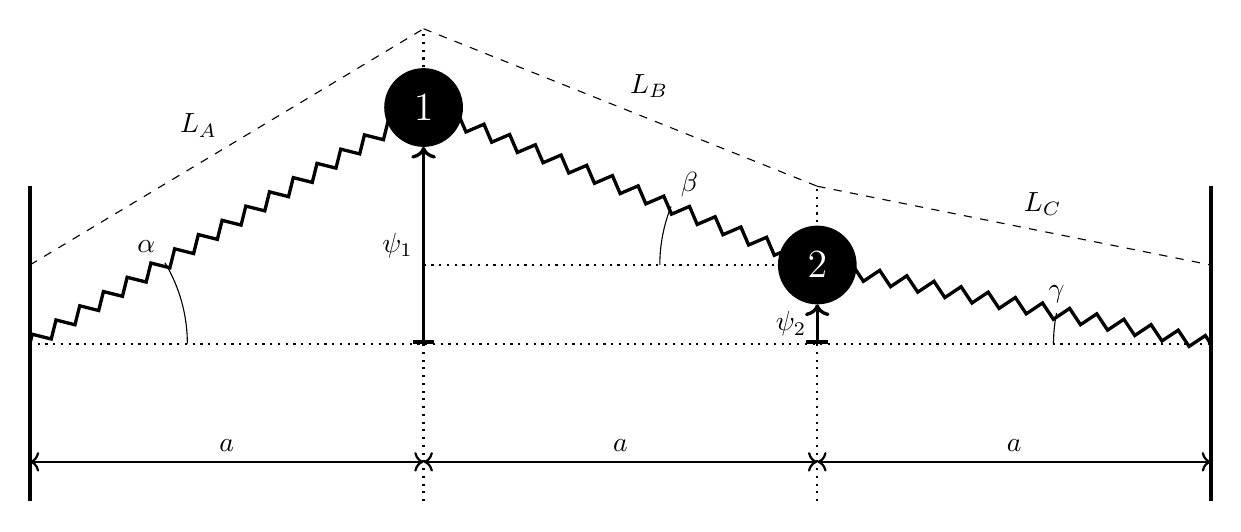
\begin{tikzpicture}

\coordinate (A) at (-2.5,3);
\coordinate (B) at (2.5,1);

\draw[ultra thick](-7.5,-2)--(-7.5,2);
\draw[ultra thick](7.5,-2)--(7.5,2);

\draw[dotted,thick](-2.5,-2)--($(A)+(0,1)$);
\draw[dotted,thick](2.5,-2)--($(B)+(0,1)$);
\draw[dotted,thick](-7.5,0)--(7.5,0);

\draw[very thick,|->,](-2.5,0)--node[anchor=east]{$\psi_1$}($(-2.5,0|-A)-(0,0.5)$);
\draw[very thick,|->,](2.5,0)--node[anchor=east]{$\psi_2$}($(2.5,0|-B)-(0,0.5)$);

\draw[<->,thick](-7.5,-1.5)--node[anchor=south]{$a$}(-2.5,-1.5);
\draw[<->,thick](-2.5,-1.5)--node[anchor=south]{$a$}(2.5,-1.5);
\draw[<->,thick](2.5,-1.5)--node[anchor=south]{$a$}(7.5,-1.5);

\draw[very thick,snake=zigzag](-7.5,0)--(A);
\draw[very thick,snake=zigzag](A)--(B);
\draw[very thick,snake=zigzag](B)--(7.5,0);

\draw[dashed]($(-7.5,0)+(0,1)$)--node[anchor=south east]{$L_A$}($(A)+(0,1)$);
\draw[dashed]($(A)+(0,1)$)--node[anchor=south west]{$L_B$}($(B)+(0,1)$);
\draw[dashed]($(B)+(0,1)$)--node[anchor=south west]{$L_C$}($(7.5,0)+(0,1)$);

\draw[dotted,thick](B-|A)--(B);
\draw(-5.5,0)arc(0:atan(3/5):2)node[anchor=south east]{$\alpha$};
\draw(5.5,0)arc(180:180-atan(1/5):2)node[anchor=south]{$\gamma$};
\draw(0.5,0|-B)arc(180:180-atan(2/5):2)node[anchor=south west]{$\beta$};

\fill(A)circle(0.5)node{\color{white} \Large {$1$}};
\fill(B)circle(0.5)node{\color{white} \Large {$2$}};

\end{tikzpicture}
\end{document}